\section{SiPM Simulation}

In addition to studying the new electronics with the test beam, we also created a SiPM simulation that takes theoretical input signals from the detector and calculates the SiPM's response~\cite{SiPMSimulation_github}. When light from the detector goes to the SiPM, a light mixer is used so that the light is spread across the pixels on the SiPM. The intensity of light on the SiPM over time is described by the so-called Y11 pulse shape, because its shape is mainly due to the Y11 wavelength-shifting fiber that takes the photons from the scintillator to the SiPMs. The Y11 pulse shape is shown in Figure~\ref{fig:Y11}. Using a mathematical representation of this pulse shape, we can simulate how light is shined on the SiPM. We can then create a virtual SiPM that has an accurate geometric representation of the pixels. Each of these virtual pixels could be activated by the incoming Y11 light pulse and would respond by firing off a set amount of charge like an actual SiPM. When these pixels are activated, they also have a certain probability to activate neighboring pixels, which simulates the crosstalk of the SiPM. Each pixel also has a recharge rate such that, if hit in rapid succession, it will fire with a reduced amount of charge, which emulates the saturation effect. In this simulation we can easily adjust the number of input photons and obtain details of the SiPM response. We can also turn on and off different features of the SiPM in order to see how significant individual effects are. Using the simulation, it is simple to change the input to model different situations and gather large quantities of data. The accuracy of this simulation is heavily dependent on the data we input into it.

Since the program can simulate the nonlinearity effects of the SiPM, we can use theoretical inputs to the SiPM to study its effects. As the Y11 pulse shape does not change with the number of photons, to simulate a higher energy particle, we simply need to increase the total number of photons in the incident pulse. The output of the virtual SiPM is normalized so that if the SiPM were a completely linear device, its output ``charge'' should exactly equal the number of input photons.

\begin{figure}
\centering
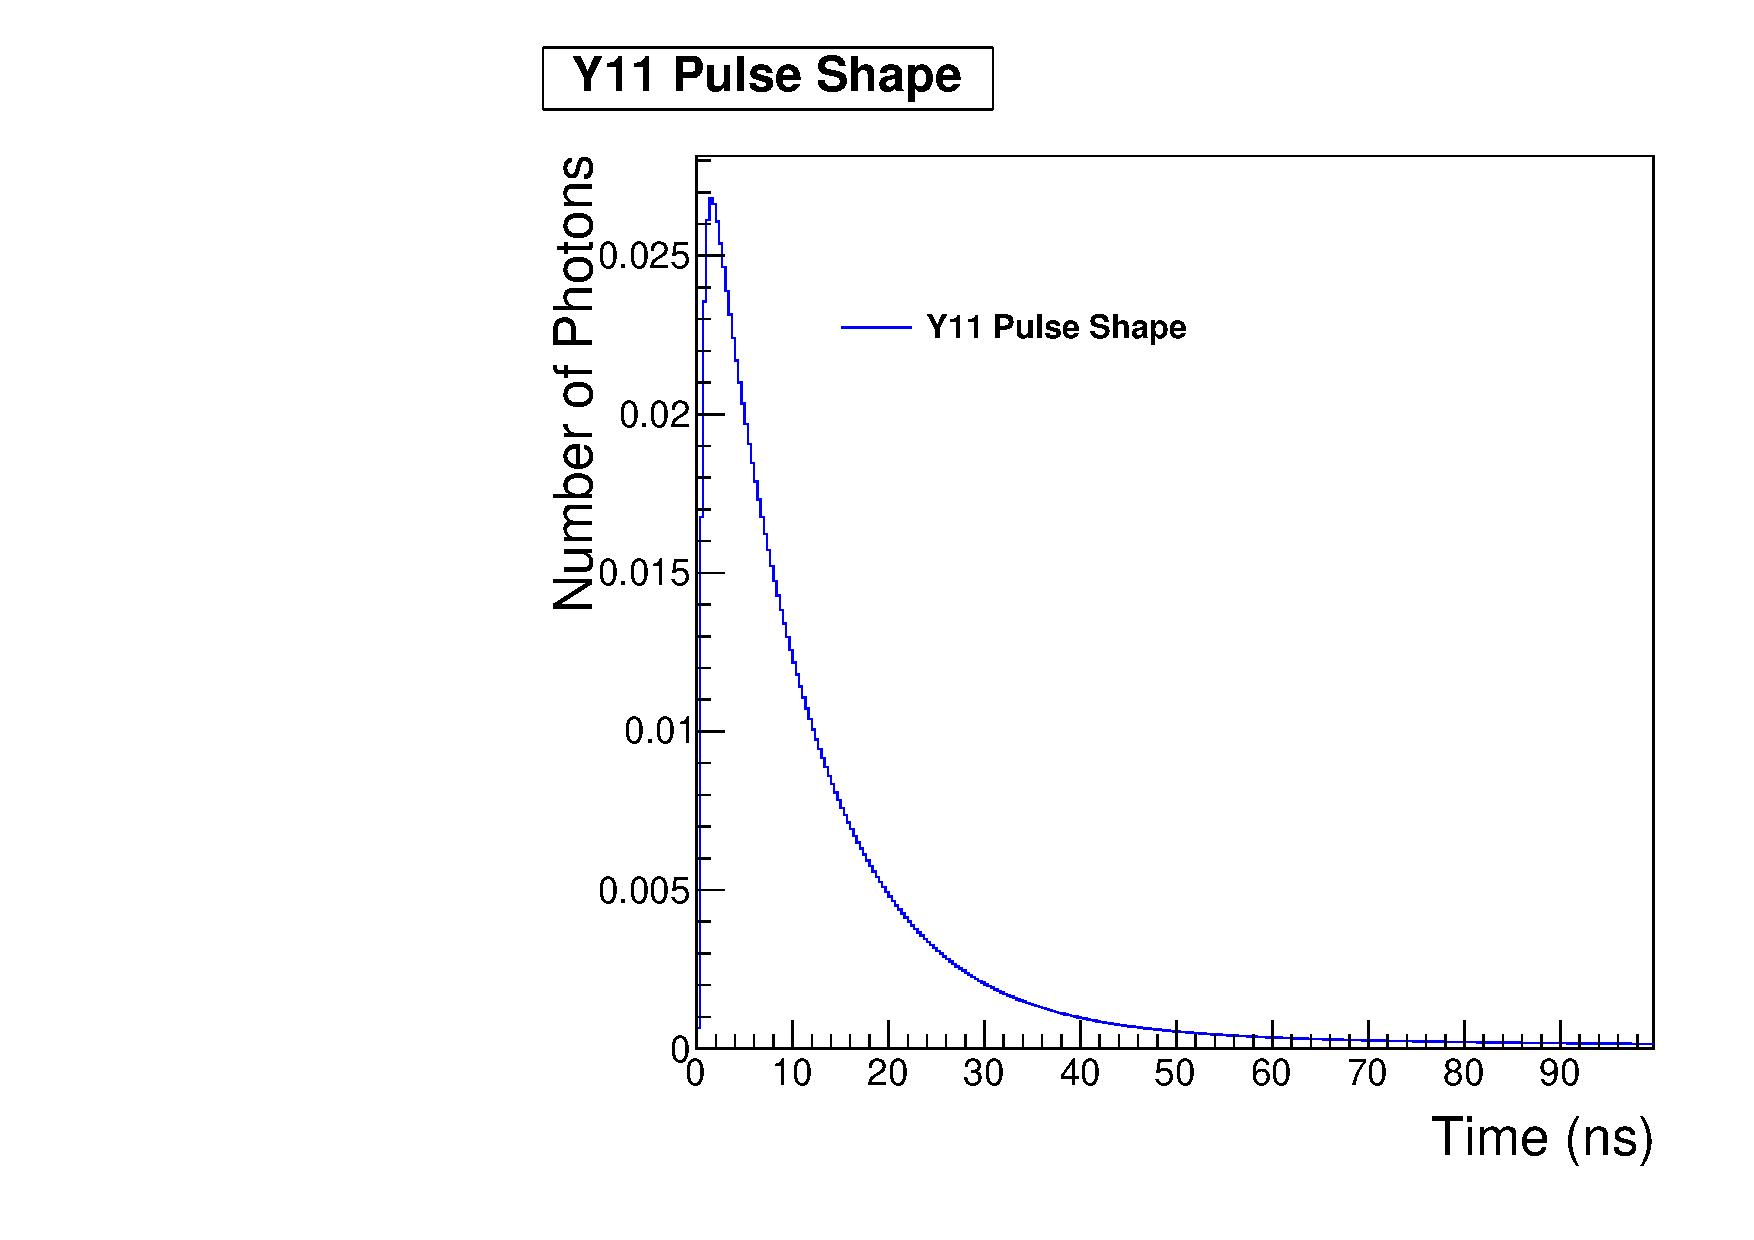
\includegraphics[width=0.8\linewidth]{Figures/Y11.pdf}
\caption{The Y11 pulse shape used in the SiPM simulation.}
\label{fig:Y11}
\end{figure}

\section{Simulation Analysis}

To do the analysis using the SiPM simulation, we simply measure the total output of the SiPM over a light pulse and compare it to the number of input photons. Since there is a degree of randomness, we will use the average pulse over several inputs. Compared to using test beam data, the analysis with the simulation is simple. In the test beam, the energy of the particle is spread over several SiPMs, while in the simulation we have very fine control of the input energy to the single SiPM. With a plot of input number of photons vs.\ SiPM output charge, we then create a correction curve that is necessary to make the graph linear. This is a process for doing a nonlinearity analysis using test beam data so that we can compare the two correction curves to see if there is agreement. With other analyses it is common to simply divide out the crosstalk. Given that there is a $15.4\%$ chance of crosstalk with a large signal of several thousand photons, it is assumed that $15.4\%$ of the signal from the SiPM is due to crosstalk, so that charge is ignored. This means the majority of the effects that the correction curve is compensating for is saturation. Figure~\ref{fig:SimNon} shows the nonlinearity obtained from the simulation.

\begin{figure}
\centering
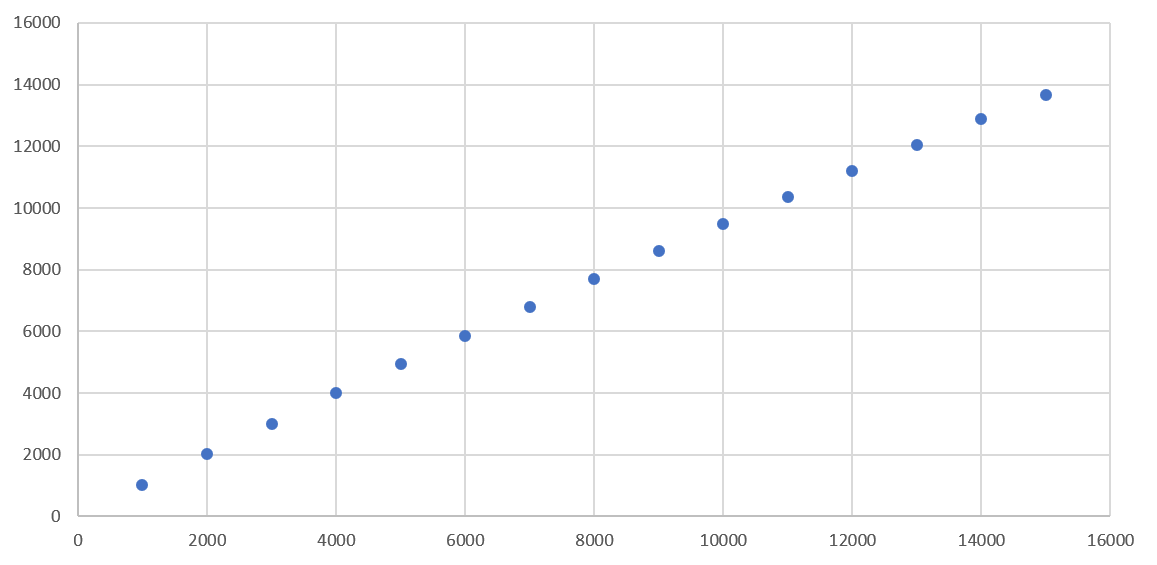
\includegraphics[width=0.8\linewidth]{Figures/SimNon.png}
\caption{The number of incident photons vs.\ output charge of the SiPM simulation with a $y=x$ line for reference. Given the units of the simulation, a perfectly linear device would have all data points falling on the $y=x$ line, but as shown, as the number of incident photons is increased the data points fall short of this line.}
\label{fig:SimNon}
\end{figure}

To be sure the simulation is designed correctly, it is useful to compare things such as nonlinearity to the actual SiPM. Figure~\ref{fig:NonLin} shows the nonlinearity of the SiPM from shining a laser directly on the SiPM. Figure~\ref{fig:Cor} shows a similar plot constructed using the simulation. There is significant disagreement between these two sets of data.

\begin{figure}
\centering
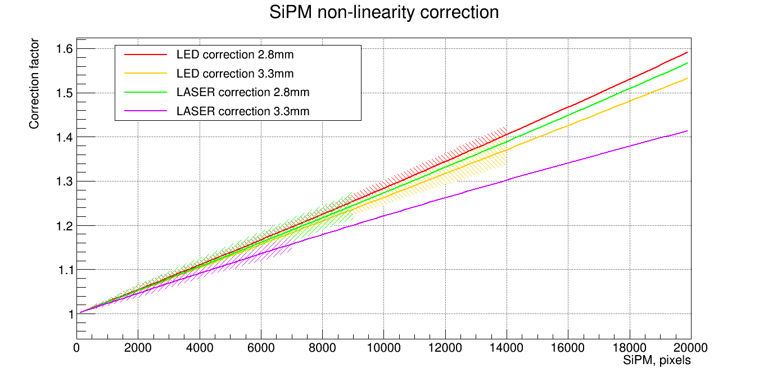
\includegraphics[width=\linewidth]{Figures/LaserNonLin.png}
\caption{The SiPM nonlinearity correction factor vs.\ number of pixels fired. The correction factor is the number the output needs to be multiplied by in order to obtain a linear output value. This means a perfectly linear device would always have a correction factor of 1. This data was obtained by shining a laser directly on the SiPM.}
\label{fig:NonLin}
\end{figure}

\begin{figure}
\centering
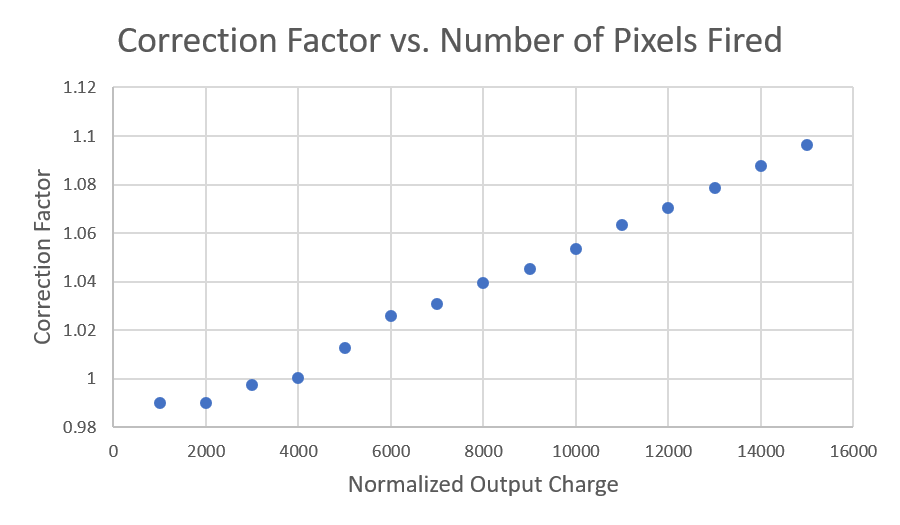
\includegraphics[width=\linewidth]{Figures/CorFac.png}
\caption{The correction factor vs.\ number of pixels fired. The correction factor is the value that the output needs to be multiplied by in order to obtain a linear output value. This means a perfectly linear device would always have a correction factor of 1. These data was obtained from the SiPM simulation.}
\label{fig:Cor}
\end{figure}

One effect of saturation that is less understood and harder to implement is that the pixels can sometimes recharge faster. This effect is due to the QIE chips in the readout modules which, in addition to taking and processing the charge from the SiPMs, also supply the charge that recharges the capacitors for each individual pixel. The capacitors for the pixels recharge exponentially, as expected from normal RC circuits. Normally the time constant for the capacitors is about 9~ns, which means the capacitor is completely recharged after 20~ns, but this is when the SiPM is outputting a very low amount of charge to the QIE chips. When the SiPM is outputting more charge, the QIE chips supply more charge to the SiPM, recharging the pixels faster. When the pixels recharge fast, they fire off charge closer to the maximum charge even when hit in rapid succession. This means the effects of saturation are diminished when the output charge of the SiPM increases. The effect of different recharge time constants for the pixels can be seen in Figure~\ref{fig:trc}.

\begin{figure}
\centering
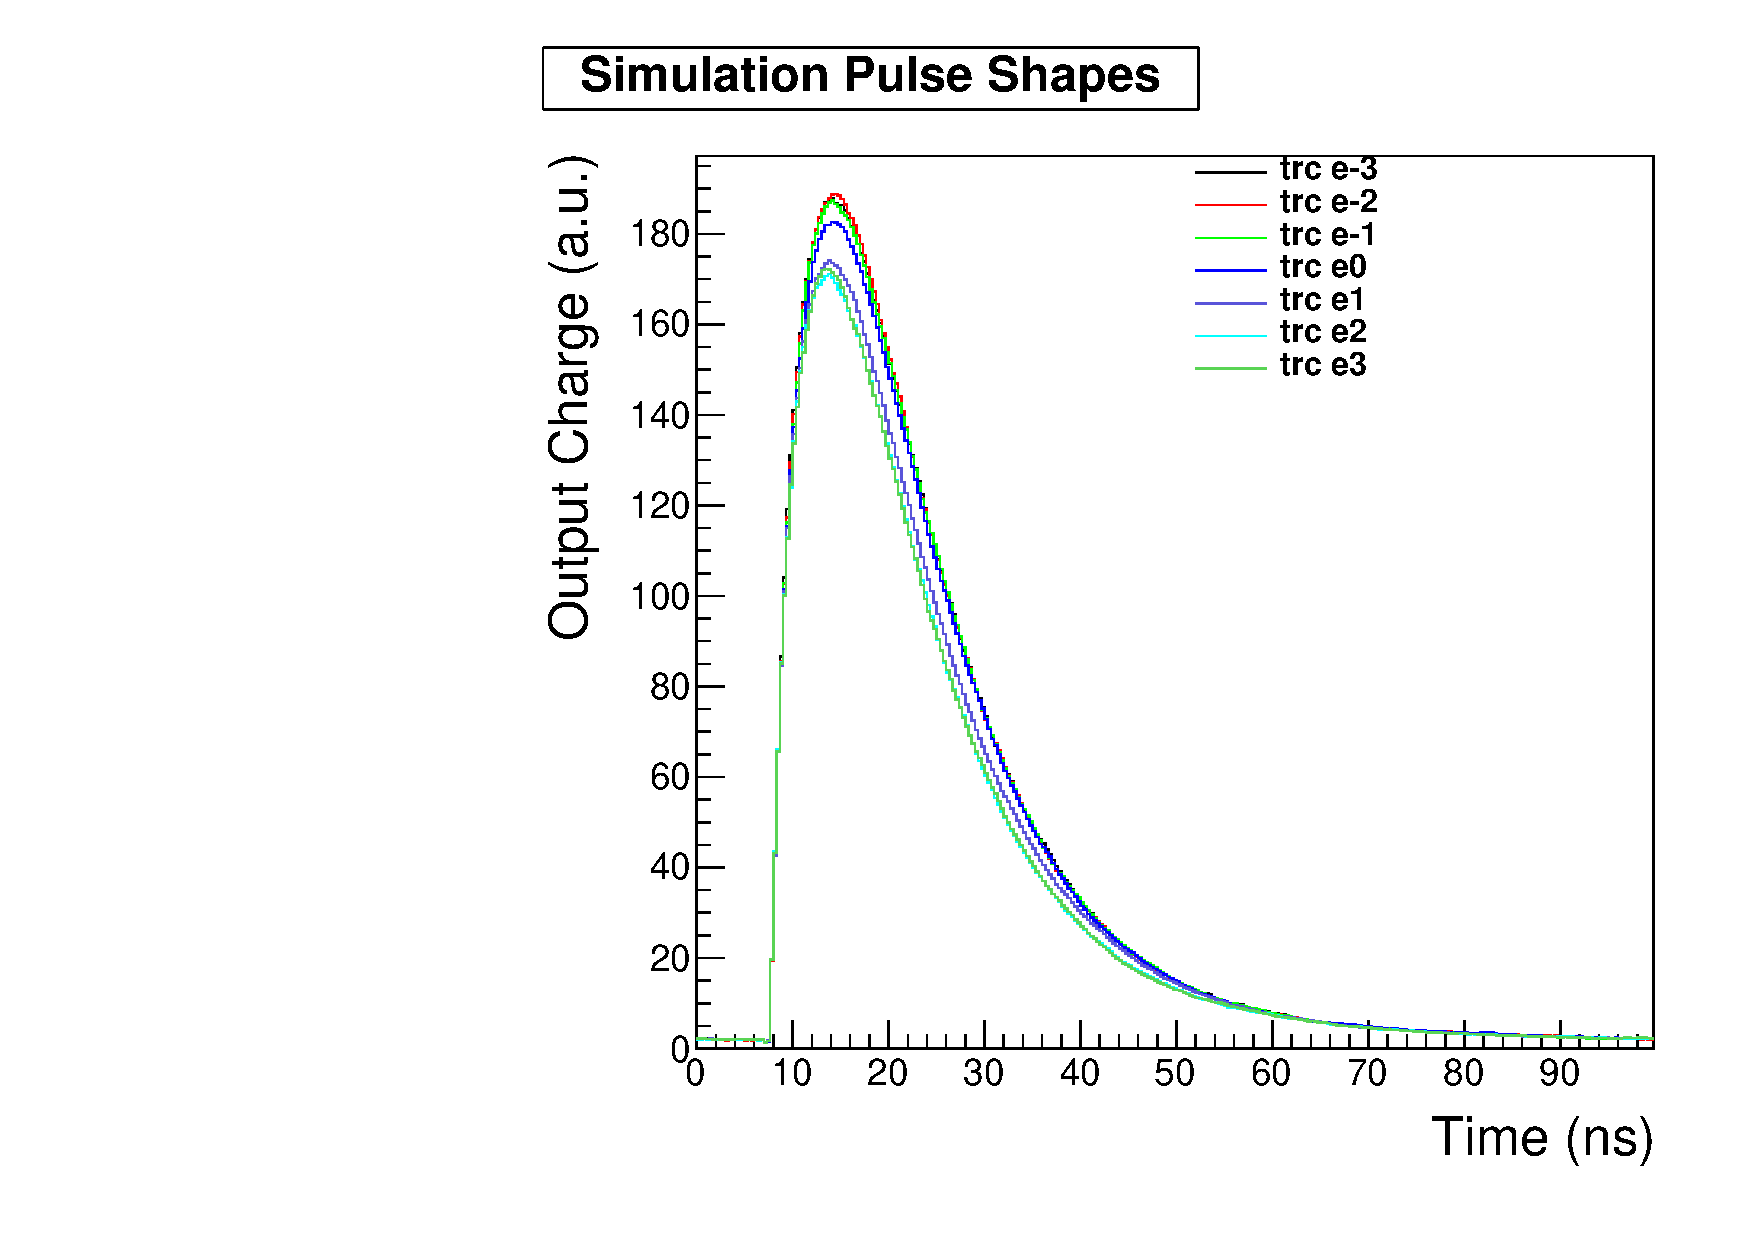
\includegraphics[width=0.8\linewidth]{Figures/trc.pdf}
\caption{Output pulses of the SiPM simulation with 10,000 incident photons comparing the effect of changing the recharge time constant on the pixels. The TRC value is the recharge time constant ranging from $10^{-3}$ to $10^3$.}
\label{fig:trc}
\end{figure}

Using the simulation we can also look at the pulse shape of the SiPM. This pulse shape should theoretically be the same as that obtained from test beam data. One of the main things that is interesting to look at is ``does the pulse shape change significantly with a change in input energy?'' As shown is Figure~\ref{fig:SimPul}, the output pulse shape does not significantly change with different energies.

\begin{figure}
\centering
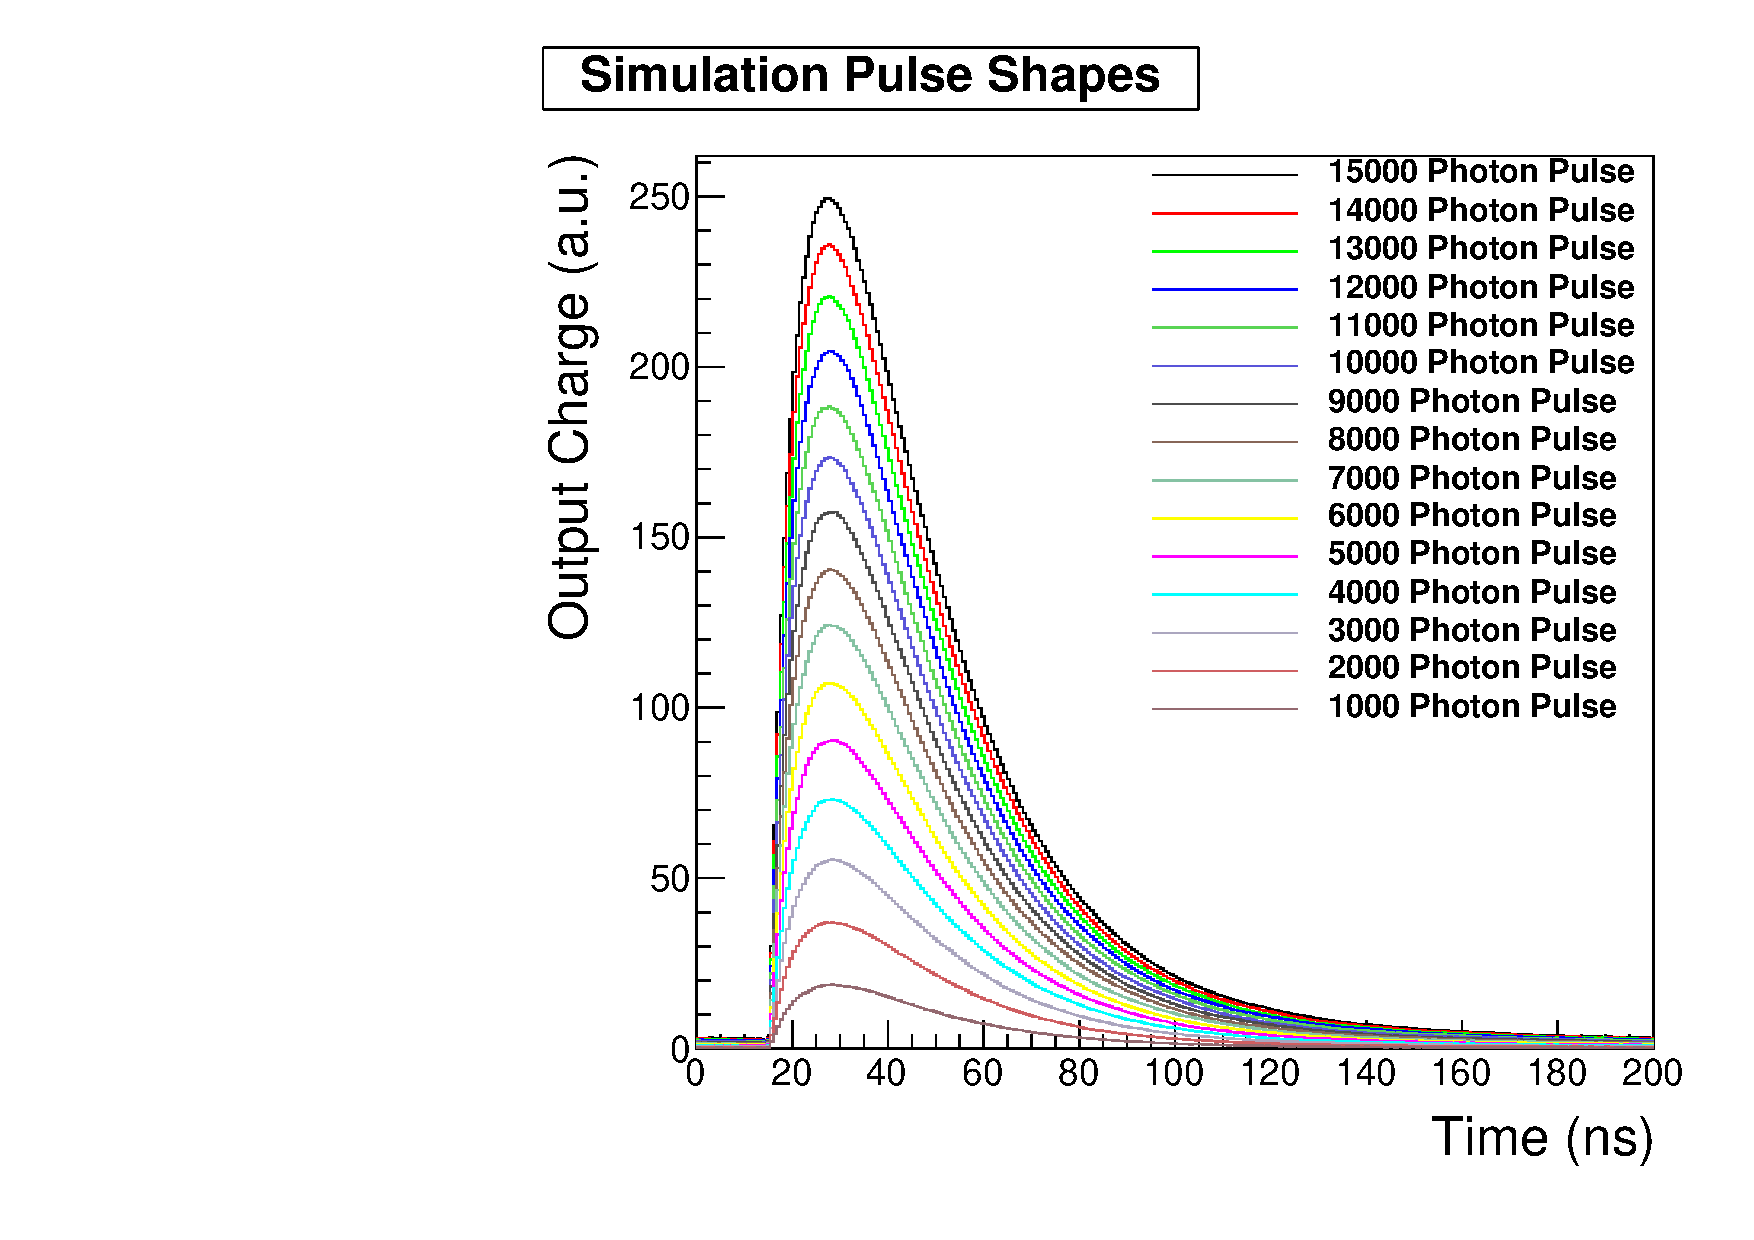
\includegraphics[width=0.8\linewidth]{Figures/SimPul.pdf}
\caption{Pulse shapes from the SiPM simulation. They are overlaid on top of each other to highlight any differences from increasing the input photon count.}
\label{fig:SimPul}
\end{figure}

We can compare the pulse shape from the simulation to the one obtained from test beam data. These pulses are expected to be the same. For comparison we simply plot the two pulse shapes on top of each other and see if there are any major differences. To minimize the interference of other effects such as nonlinearity, we can compare pulses from similar output charge. Using the conversion ratio of 40~fC to 1 photon, we can compare pulses from the same charge range. We compare the pulse shape from the charge range 10,000--29,000 fC to one from the simulation results from 500 input photons. Figures~\ref{fig:1comparison_together} and~\ref{fig:2comparison_together} show these comparisons. While they do have the same basic shape, there are some differences --- mostly, the simulation is much narrower in the base.

\begin{figure}
\centering
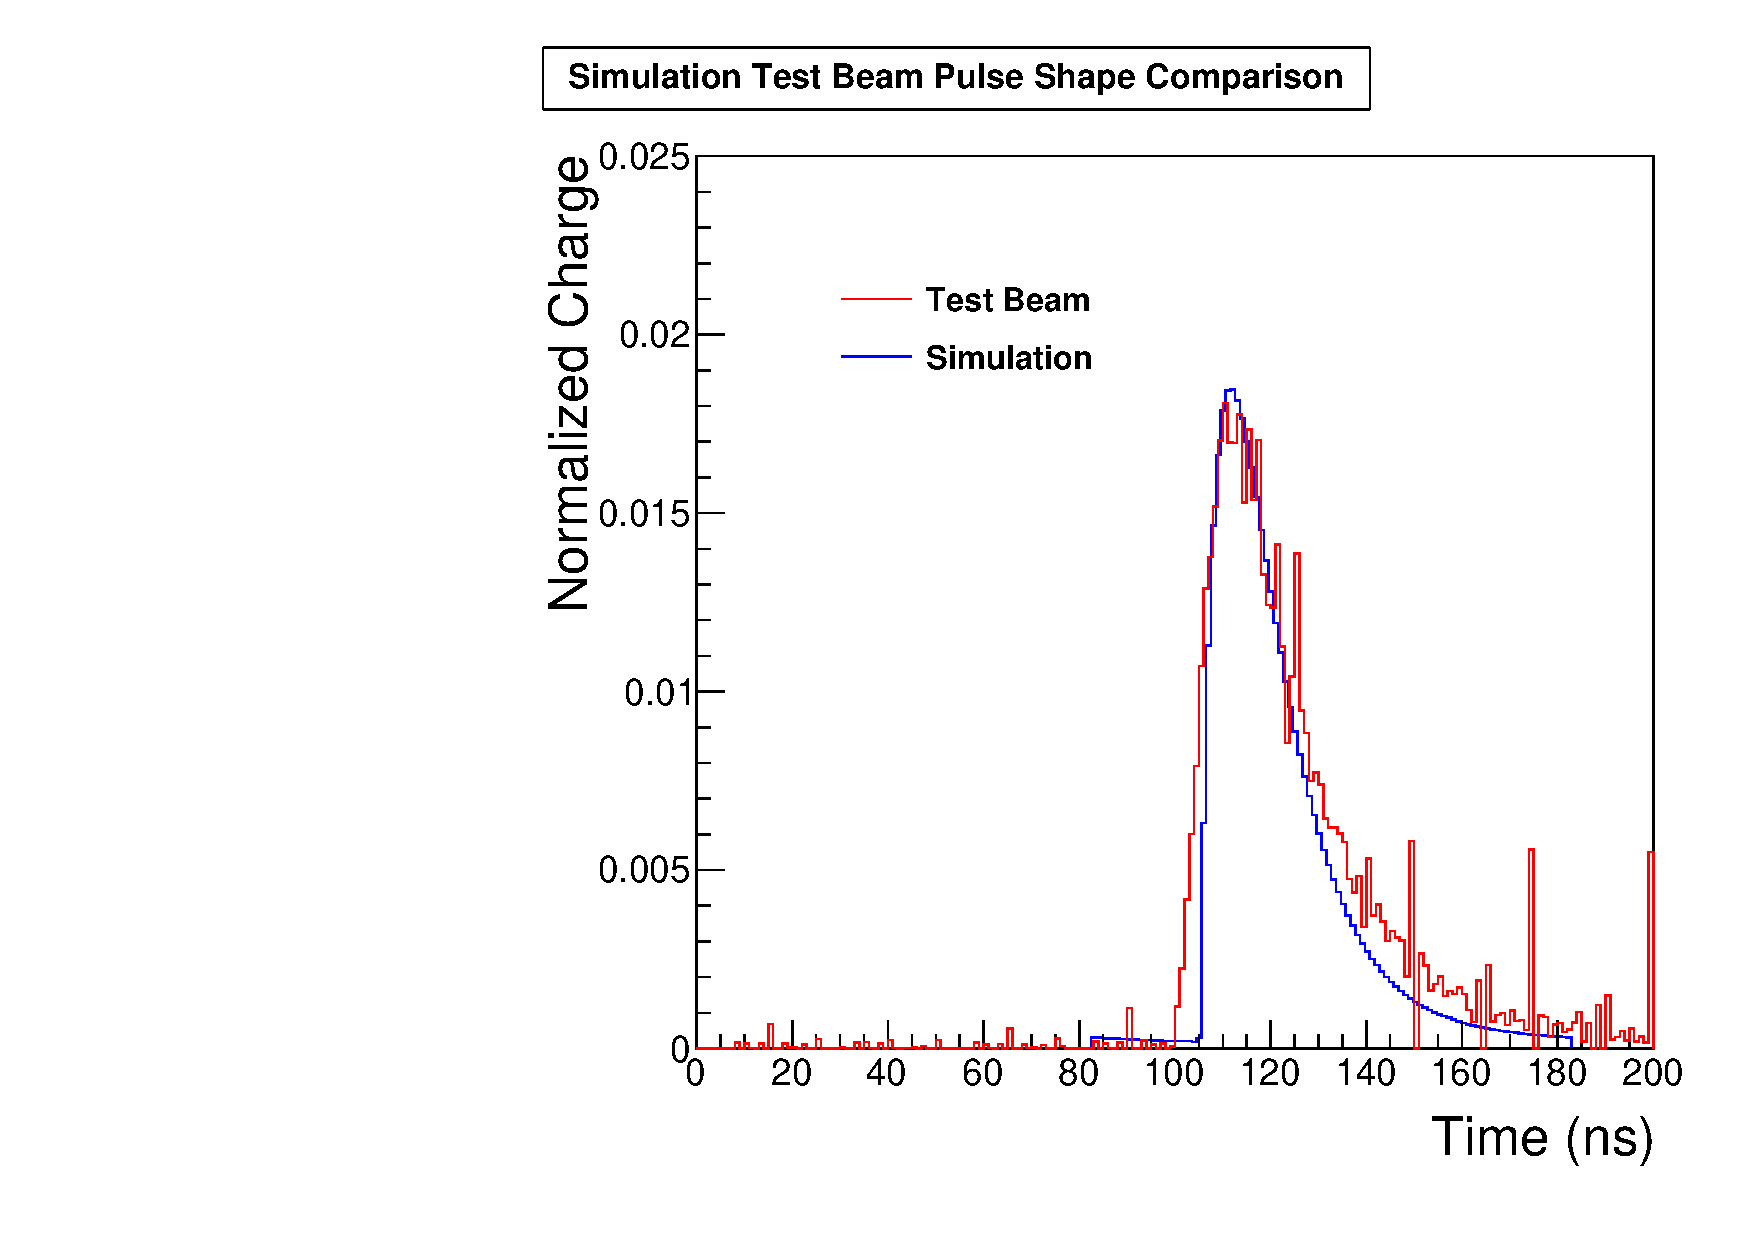
\includegraphics[width=0.495\linewidth]{Figures/10Comparison.pdf}
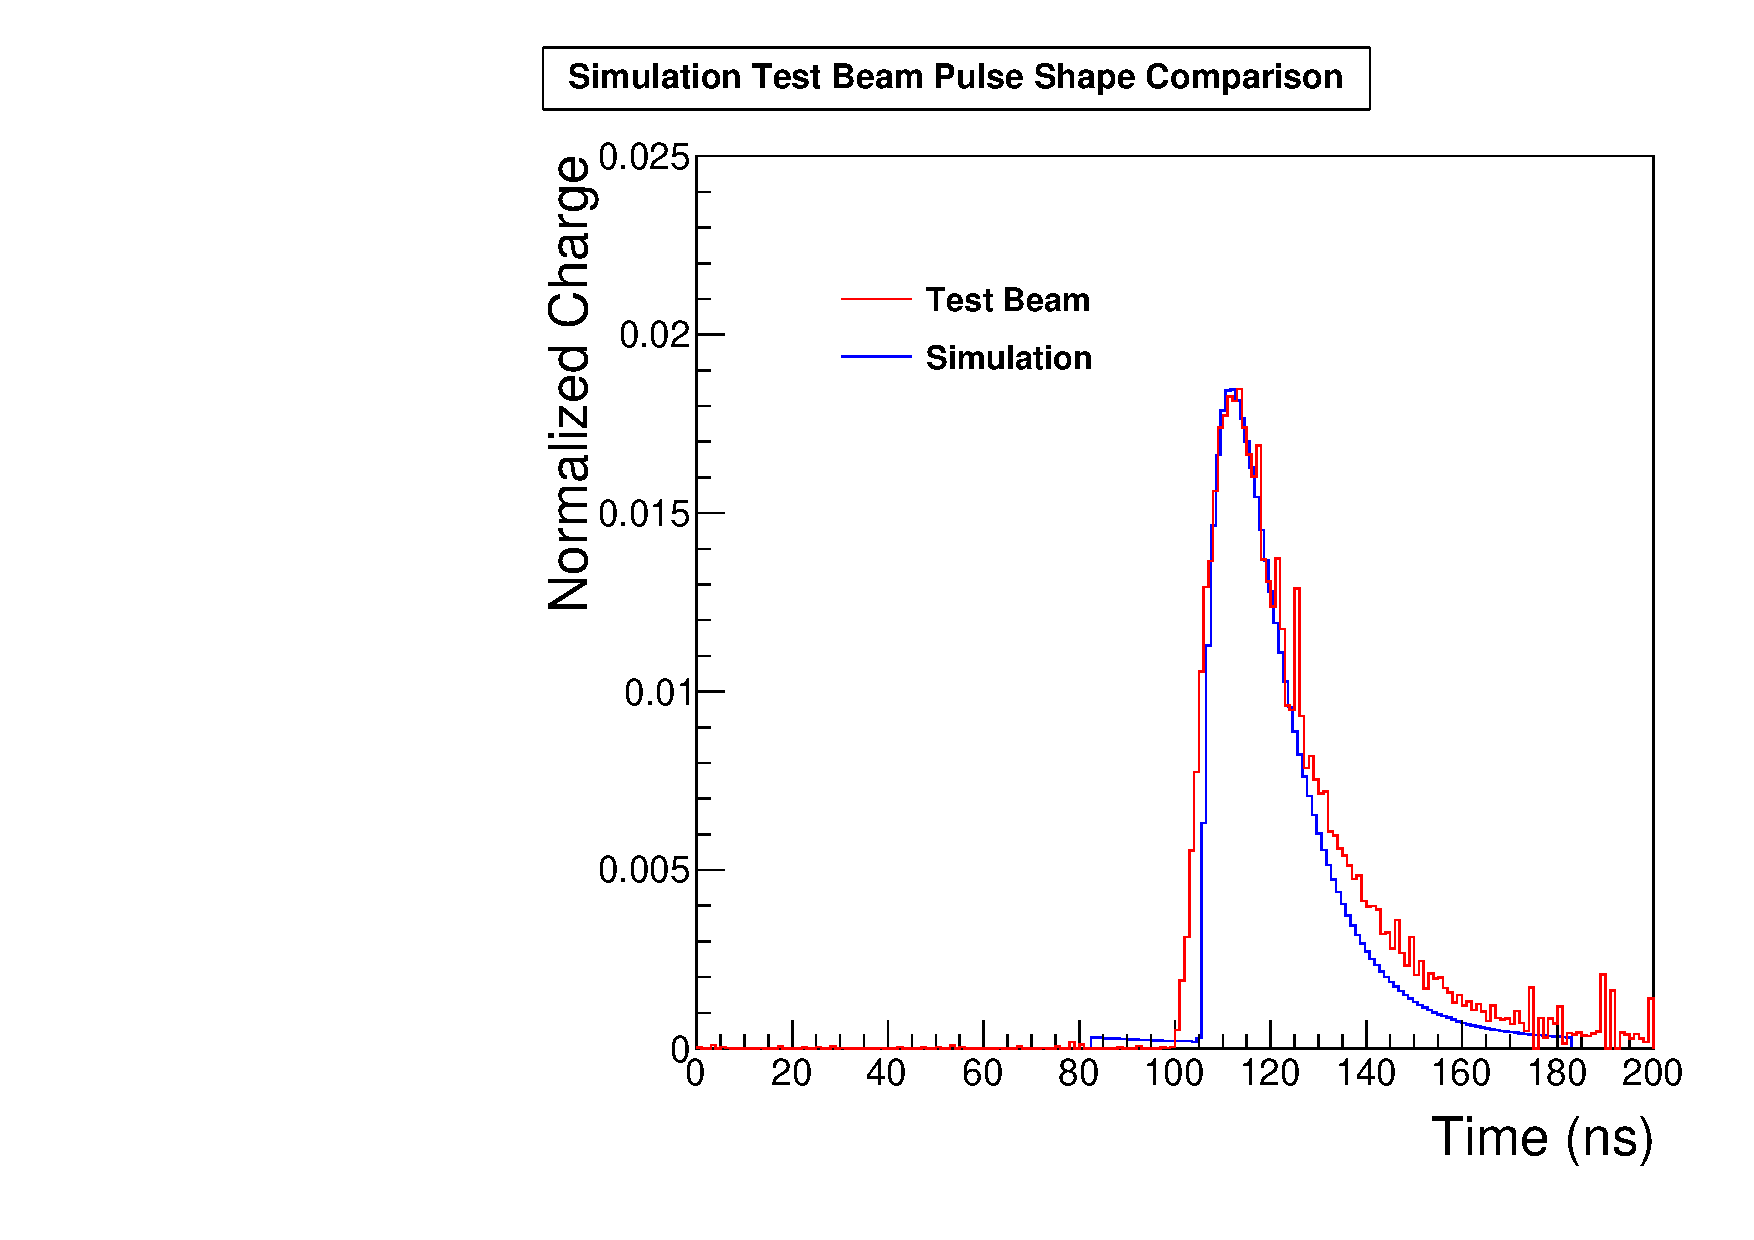
\includegraphics[width=0.495\linewidth]{Figures/29Comparison.pdf}
\caption{The pulse shapes from the simulation and the test beam data, overlaid for comparison purposes. On the left the charge range is 10,000--29,000 fC and on the right it is 29,000--50,000 fC.}
\label{fig:1comparison_together}
\end{figure}

\begin{figure}
\centering
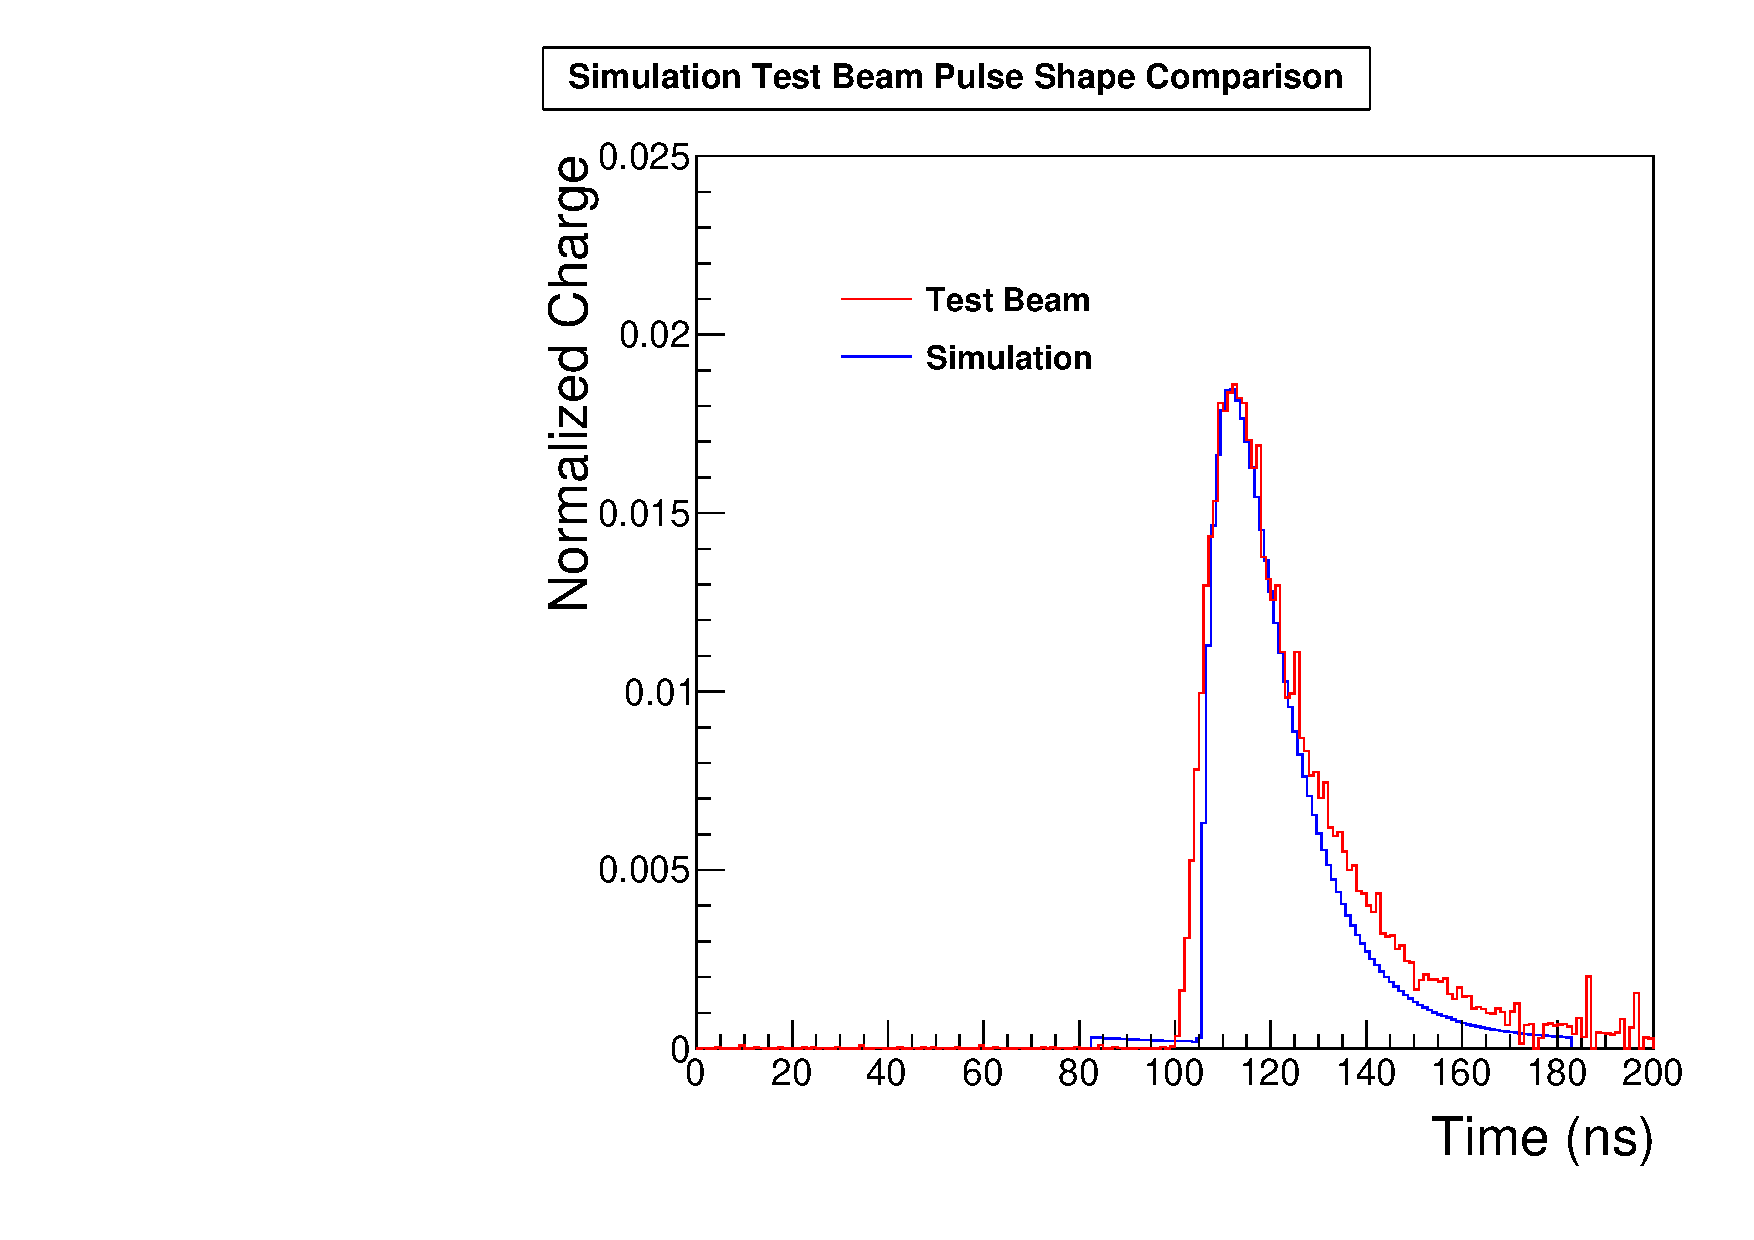
\includegraphics[width=0.495\linewidth]{Figures/50Comparison.pdf}
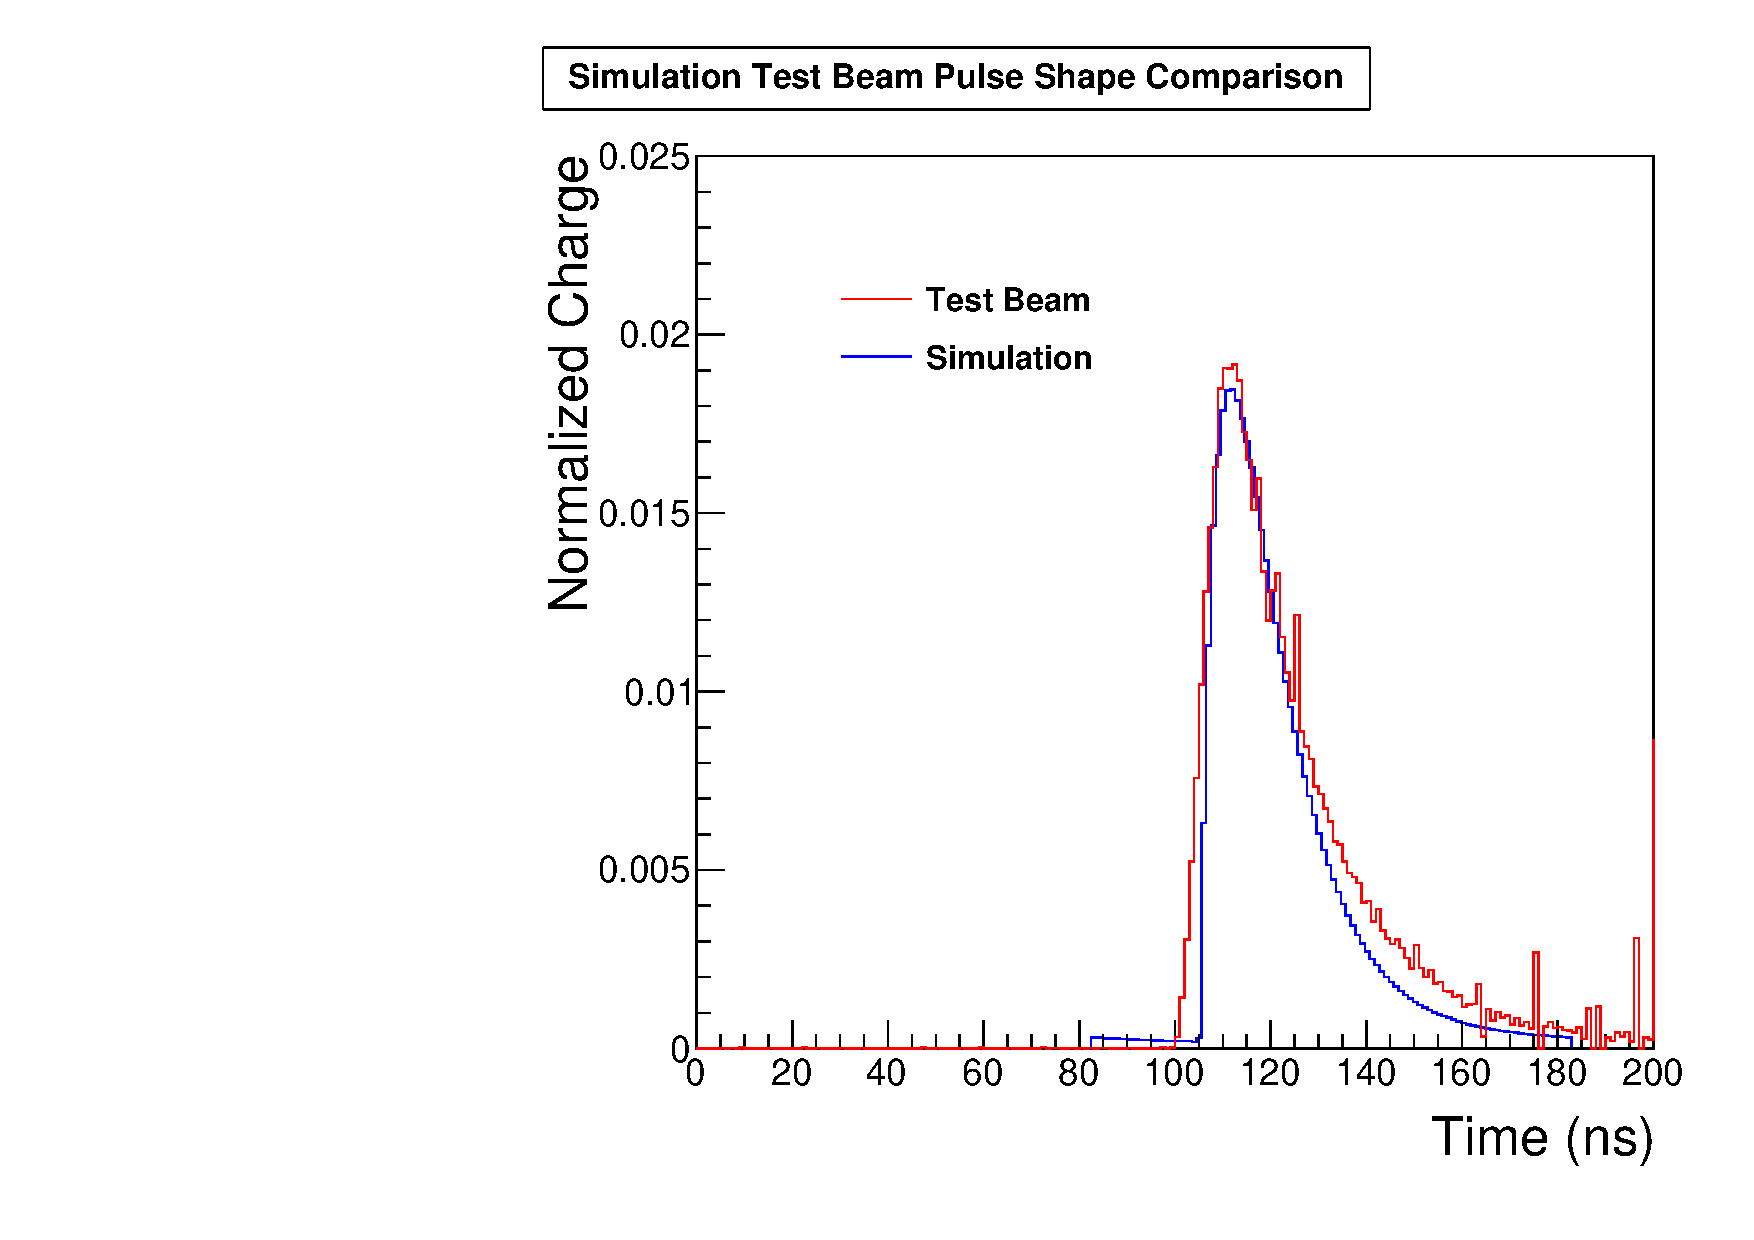
\includegraphics[width=0.495\linewidth]{Figures/80Comparison.pdf}
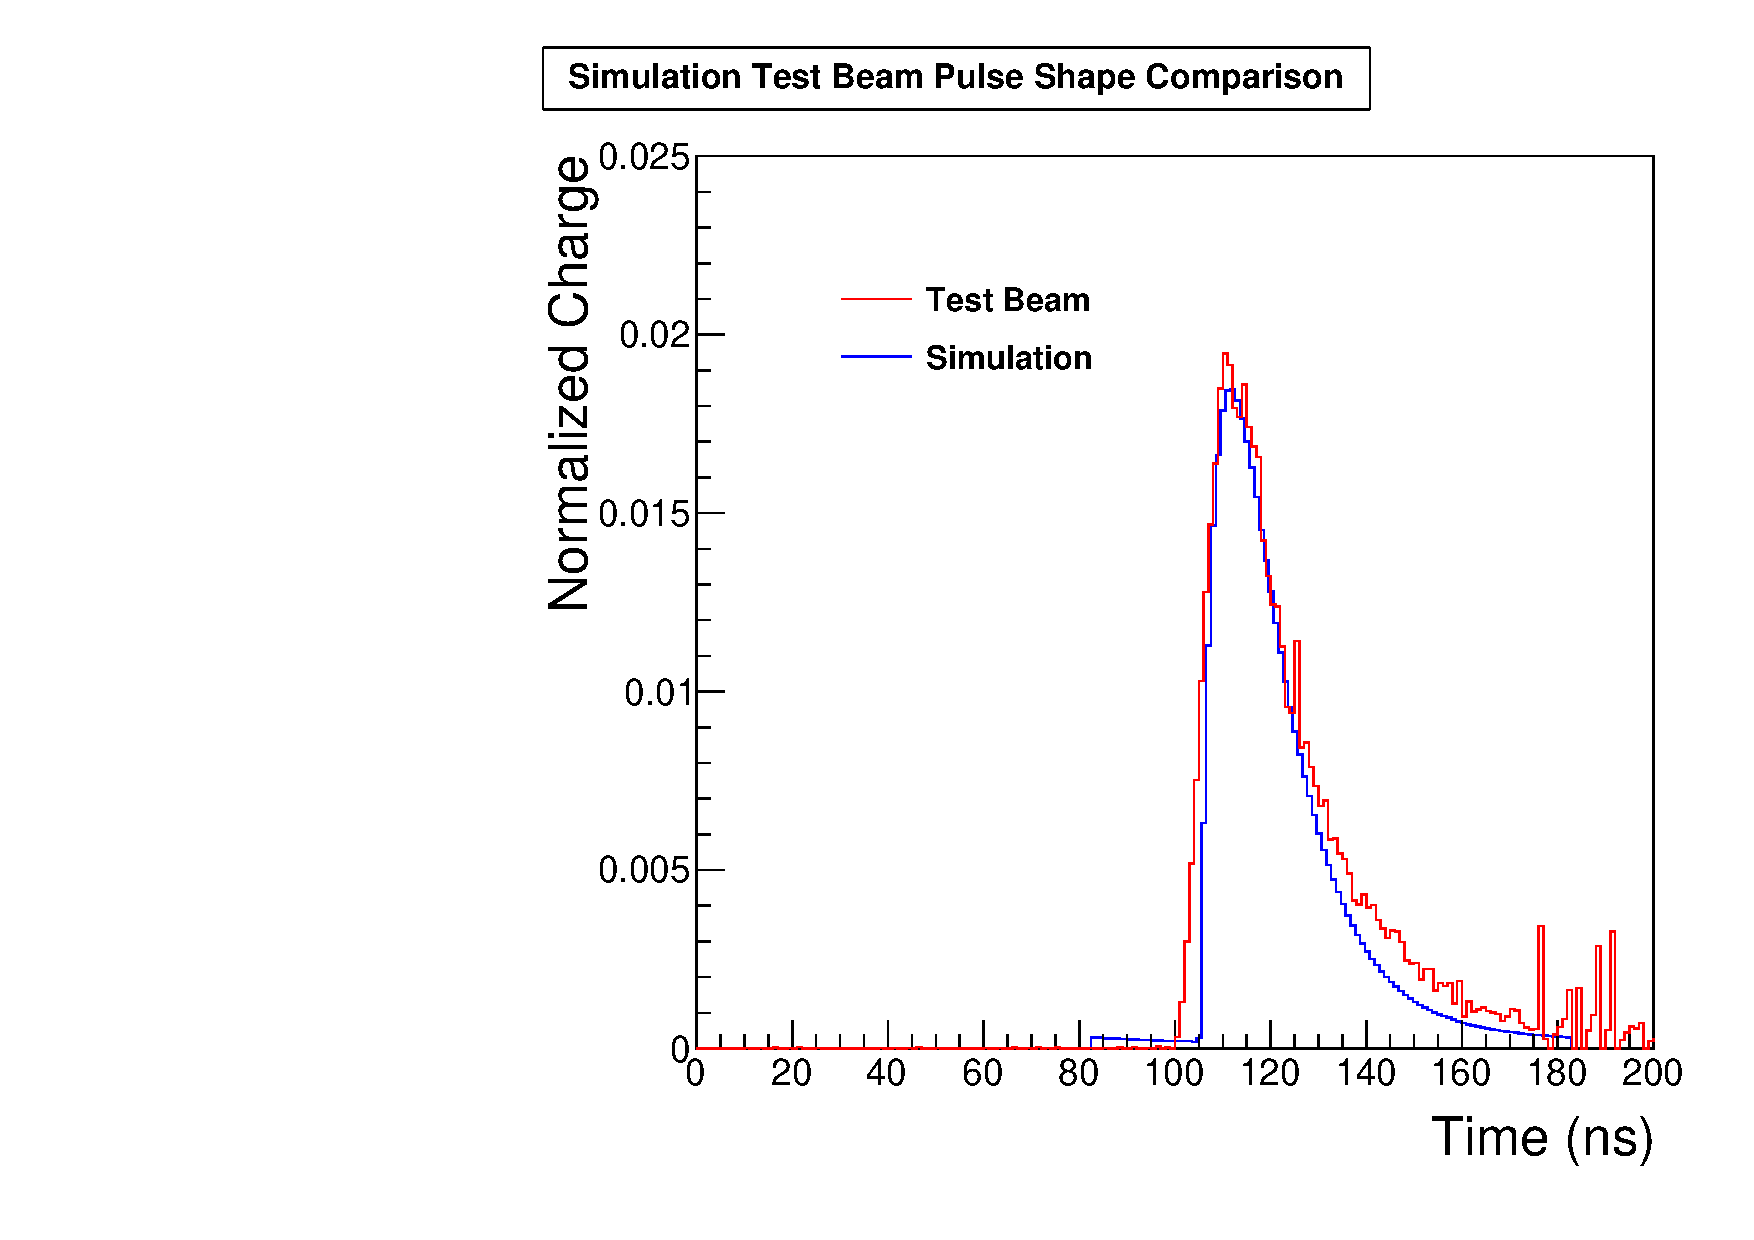
\includegraphics[width=0.495\linewidth]{Figures/125Comparison.pdf}
\caption{The pulse shapes from the simulation and the test beam data overlaid for comparison purposes. On the left the charge range is 50,000--80,000 fC, on the right it is 80,000--125,000 fC, and on the bottom it is 125,000--168,000 fC.}
\label{fig:2comparison_together}
\end{figure}

\section{Summary}

The simulation is a useful illustration for how the SiPM works, and it can be easily adjusted for future modifications. Some of the plots used in this thesis to explain how a SiPM works were created using this simulation. The analysis of the simulation, however, shows that there are still some flaws with the simulation. The pulse shape comparison shows that the simulation shape is narrower in the base than the measured pulse shape. In addition, the nonlinearity in the simulation is much smaller than measurements made using an actual SiPM. The reasons for these discrepancies are still being investigated, but there are several leads. Among them are the changing recharge times and other effects such as the scintillator tiles and QIE chips not yet taken into account in the simulation. 